\documentclass[aps,prb,floatfix,twocolumn,twoside,english]{revtex4-1}

\usepackage[dvips]{graphicx}
\usepackage[latin1]{inputenc}
\usepackage[T1]{fontenc}
\usepackage{amsmath}
\usepackage{verbatim}
\usepackage{epsfig}
\usepackage{babel}
\usepackage{dialogue}

\begin{document}

\title{Undergraduate students' challenges when modeling physics computationally}

\author{Simen A. S{\o}rby}

\affiliation{Department of Physics, University of Oslo, N-0316 Oslo, Norway}

%\author{Carl Angell}

%\affiliation{Department of Physics, University of Oslo, N-0316 Oslo, Norway}

%\author{Morten Hjorth-Jensen}

%\affiliation{Department of Physics, University of Oslo, N-0316 Oslo, Norway}

\date{\today}


\begin{abstract}

In later years, computational perspectives have become essential parts in several of the University of Oslo's natural science studies. In this paper I discuss some main findings from a qualitative study of the computational perspectives' impact on the students' work with their first course in physics -- mechanics -- and their learning and meaning making of its contents. Discussions on the students' learning of physics are based on the sociocultural theory, which originates in Vygotsky and Bakhtin, and subsequent physics education research. Results imply that computational assignments' greatest challenge is their combined use of students' knowledge from earlier separated contexts. Making use of informatics, numerical and analytical mathematics and conceptual understanding of physics in one big package, appears as a clear challenge for the students. I also observe a lack of awareness considering the limitations of physical modeling. The students seem to need help becoming aware of using the sufficient knowledge and system of conception, or ``tool set'', for the different tasks at hand; they need help creating a plan for their modeling and to become aware of its limits. In light of this, I propose an instructive and dialogic text as grounds for the exercises, in which stress is laid on specification, clarification and elaboration, to be of potential great aid for students who are new to computational modeling.

\end{abstract}

\maketitle

\section{Introduction}

Both computers and the great span in numerical methods for mathematical computations have gradually evolved due to scientific research with its endless stream of new questions and technology's seemingly unstoppable advancements. This development has in turn caused significant changes in a physicists expected tasks in his or her line of work, be it either in research or industry. As a consequence, computational perspectives have become essential parts in several of the University of Oslo's natural science studies, including the Physics, Astronomy and Meteorology branch, which is the subject of this paper. These changes are the results of some enthusiastic people working with a project called Computers in Science Education (CSE) at the University of Oslo.\cite{CMACSE} The goal of this project is to develop a unified computational perspective on undergraduate teaching programs across course and departmental boundaries.

The students will in their first semester at the University gain important insight in both analytical and numerical mathematics, as well as the programming language Python. The knowledge and skills they build up during this semester is fundamental for working with courses further up in the system. For the physics students in particular, the first semester will lay the foundation for modeling physical systems and phenomena with computational perspectives in their second semester and their first course in physics, mechanics. Computational perspectives are integral parts of this course and stand side by side with traditional physics theory. To accomplish this, new course material has been developed -- including textbook material and exercises -- which incorporates these new aspects as a natural part of the curriculum. The new exercises involve writing program codes in Python to simulate a broad range of physical systems on the computer. 

Since the CSE-project has started to bear fruits, it was made possible in 2008/2009 to carry out a study on how these new aspects impacts the students work with and learning of physics. The goal of the study was to gain insight into students' work with compulsory assignments in the mechanics course with regards to its computational perspectives. The main focus was looking into whether the students were well prepared to carry out these assignments after having gone through their first semester and whether these assignments arrange for a good way of physics. What challenges might the students' encounter in their learning situation when working with the computational aspects of the mechanics course? What might be done to help the students overcome these challenges?

In section \ref{sec:mechanics_course} of this paper, I will outline a typical student assignment followed by the general way of tackling its computational parts. Section \ref{sec:theory} will present the theoretical framework needed for discussing the students' learning and meaning making of the course content, and section \ref{sec:method} will briefly outline the method used for gathering data. Finally, in sections \ref{sec:results} and \ref{sec:implications}, I will present and discuss some possible challenges the students might face in the mechanics course. I will also, from a sociocultural point of view, discuss possible ways of helping the students overcome these challenges.

\section{A course in mechanics with computational perspectives}
\label{sec:mechanics_course}

\subsection{An example of a student assignment}

This assignment regards a ball with mass $m$ in a spring moving in a vertical plane -- an elastic pendulum motion. The force on the rope is described with a spring model with spring constant $k$ and equilibrium length $L$. The assignment starts out with asking the students to draw a free-body diagram and to show that the forces in play can be written as
\begin{equation}
 \sum \vec F = -mg \hat j - k(r-L) \frac{\vec r}{r}, \nonumber
\end{equation}
\noindent where $\vec r$ determines the position of the ball and $g$ is the gravitational acceleration.

Some more analytical exercises are given, like calculating analytically what the position will be if the velocity is zero. Doing experiments and playing around with the physical system using only analytical mathematics might, however, be quite cumbersome (and difficult), so a program code for describing the motion of the ball is asked for. The challenge for the students is to decompose the forces and to implement them into the program code correctly. When the program is up and going, the students are asked, among other things, to experiment with the spring constant, $k$, and write down what they think might be the limitation of this modeling approach.

\subsection{Solving ordinary differential equations with Euler's method}

After their first semester, the students should know how to use Euler's method to approximate the solutions to first order ordinary differential equations on the form $y'(t) = f(t,y(t))$. A typical physics problem the students meet in their second semester mechanics course, can be described with Newton's 2. law, which is an ordinary differential equation of \textit{second order}. After introducing the variable $v(t)$ with the relation $v(t) = x'(t)$, we get a set of \textit{coupled first order} differential equations, which may be approximated with Euler's method as follows:
\noindent 
\begin{subequations}
\begin{align}
  v(t+h) &= v(t) + \frac{1}{m}\sum F(t,x(t),v(t)) \cdot h \nonumber \\
  x(t+h) &= x(t) + v(t) \cdot h \nonumber
\end{align}
\end{subequations}

In the students' program code, after declaring constants, arrays (with length $n$) and initial conditions, the essential code for computing the approximated solution can be seen below. Here, as we run through the arrays, the sum of forces divided by mass is calculated in advance (and recognized as $a$) to ease readability. Also, the more common notation of $dt$ is used for the step length. The elapsed time is updated in the end of each step.

\begin{small}
\begin{verbatim}
   for i in range (n-1):
       a[i] = F(t[i],x[i],v[i])/m
       v[i+1] = v[i] + a[i] * dt
       x[i+1] = x[i] + v[i] * dt
       t[i+1] = t[i] + dt
\end{verbatim}
\end{small}

\noindent All physical systems that can be described with a second order ODE, may be approximated with this method. The only variables that differ from system to system are the forces in play, and consequently the only basic difference from code to code is the function containing these forces.


\section{Theoretical framework}
\label{sec:theory}
\subsection{The sociocultural theory of learning and development}

The sociocultural theory emphasize that knowledge is constructed through social interaction and in a specific context, not primarily through individual processes. Knowledge is consequently situated in a historical and cultural context. The construction of knowledge involves mediation of concepts on a social plane, which can thereby be internalized by the individual.\cite{Wertsch:1985} Lev Vygotsky is widely recognized for introducing these ideas along with, what he calls, the Zone of Proximal Development (ZPD) in school children's learning and development.\cite{Vygotsky:1978} The ZPD, as defined by Vygotsky himself, \textit{is the distance between the actual development level as determined by independent problem solving and the level of potential development as determined through problem solving under adult guidance or in collaboration with more capable peers}. With guidance and collaboration being viewed as essential for learning and development, the act of imitation should as a consequence be regarded as an active process in which meaning and understanding is being constructed. When imitating someone else, the student finds himself within his ZPD on his way to master the task at hand on his own.

Regarding the social mediation of concepts, Vygotsky made a clear distinction between two types: \textit{spontaneous} and \textit{scientific}.\cite{Vygotsky:1986} Spontaneous concepts are characterized by having grounds in everyday experience and being unsystematic and strongly bound to context. Scientific concepts, on the other hand, are decontextualized and organized in a logic and hierarchic fashion. The latter are also called ``academic concepts'', i.e. concepts found in any school setting. Even though spontaneous and scientific concepts are fundamentally different in the way we encounter and learn them, they are closely related to each other in the development of concept formation: Spontaneous concepts have a development direction ``upward'' towards greater abstractness and, at the same time, they arrange for establishing scientific concepts in their ``downward'' development toward greater concreteness. The challenges teachers face is to hinder the spontaneous concepts from being overly bound to specific contexts, and at the same time hinder the scientific concepts from appearing isolated and fragmented.

When we now turn to the works of Mikhail Bakhtin, we'll take a deeper dive into \textit{how} the social mediation of concepts might take place. The main means for this process is oral or written discourse. Bakhtin pointed out that any discourse, or interplay of \textit{voices}, consists of addressed \textit{utterances} which are composed with grounds in a \textit{social language}.\cite{Wertsch:1991} A social language may be viewed as the basis of values and knowledge for the composition of the utterance; a specific point of view determined by one's social position, e.g. one's profession or other social affiliation. On the other hand, what Bakhtin refers to as ``voice'' should be compared with one's personality or consciousness. Both one's voice and uttering exists fundamentally in a social milieu and cannot be isolated from other voices, This applies for the utterance as well, however it is also being \textit{addressed}; it carries a natural expectance of a response. This may very well be an expectance of no response at all. In such a case, the utterance is regarded as \textit{authoritative}. An authoritative utterance implies that its meaning is static; it is fixed once and for all and does not encourage an interanimation of voices. The opposite of an authoritative utterance is a \textit{dialogic} utterance. In this case, the meaning is not fixed and static, but open -- it seeks new contexts to broaden its meaning. The number of such contexts is limited by the number of and heterogeneity of the voices that has the opportunity to participate in the discourse. The more contexts one can relate to a concept, and consequently the more associations one can make to it, the easier it's meaning might be to grasp.\cite{Kubli:2005} To be meaningful or of a meaning making character, the discourse should contain multiple voices which engage each other dialogically; it should strive for multivoicedness, or \textit{polyphony}, and be dialogic in nature.

Mortimer \& Scott follows the lead of Jon Ogborn and colleagues and compare, with grounds in Vygotsky's view on concept formation, learning of a school subject with \textit{building up its scientific story}.\cite{Mortimer:2003,Ogborn:1996} With regards to Bakhtin, the scientific story of physics is viewed as the physics theory expressed in terms of the ideas and conventions of the school science social language. Teaching of physics then becomes the equivalent of ``telling'' the story in its social language in a convincing way for the student, i.e. engaging the students everyday views in a topic area and developing convincing lines of argument through an interactive and dialogic dialogue.


\subsection{A conceptual understanding of physics}

A much addressed phenomenon is how students are able to solve assignments and doing well in tests without being able to show the ``correct understanding'' of the physics theory.\cite{Hestenes:1992} The students might either be lacking sufficient knowledge in a topic area or hold a faulty understanding from a scientific point of view, but still answer correctly in tests. While the first case is likely the result of rote memorization, the latter, often labeled as common sense concepts or \textit{misconceptions}, is the results of the students' having developed an individual (and faulty) understanding of the physics theory. The problem with misconceptions is that they are not arbitrary mistakes; they are firmly ingrained in the students' understanding of the concept.\cite{Hestenes:1985,Gautreau:1997} They are the tools for the students' everyday language and acts to define their way of talking and thinking.\cite{Mortimer:2003} 

These misconceptions originate in an erroneous or lacking \textit{conceptual understanding}. With grounds in the previous section, a conceptual understanding involves understanding of a subject's scientific story in its social language, i.e. grasping its scientific concepts and relating them to fruitful spontaneous concepts and other scientific concepts which may act explanatory. Showing conceptual understanding involves therefore expressing it with words. Henriksen and Angell even propose that ``to think like a physicist is to talk like a physicist''.\cite{Henriksen:2010}

Angell also proposes that instead of labeling all faulty understanding as misconceptions, one should rather view them as \textit{intuitive ideas} which might contain some degree of consistency and correct understanding.\cite{Angell:2004} Portions of the students understanding should be regarded as \textit{fragmented knowledge} which needs to be developed and refined into a more systematic scientific understanding.\cite{diSessa:1993}

Several ways of dealing with misconceptions, and consequently improving conceptual understanding, have been proposed, one being Peer Instruction.\cite{Mazur:1997} This method has been incorporated into the teaching of the students' mechanics course at the University of Oslo and involves conceptual questions (physics problems with no mathematics involved) with several answers being presented to the students during lectures. Importantly, only one answer is correct, while the others may contain more or less regular misconceptions. The main thought is that the students gain valuable insight by discussing the different answers with their neighboring students or with the lecturer.\cite{Henriksen:2010}


\subsection{Working with models in learning physics}

Traditional modeling of physical systems or phenomena involves using analytical mathematics for describing them precisely. Doing such modeling, however, requires not \textit{only} knowledge in analytical mathematics, but rather several \textit{representations} (e.g. experimental, graphical, pictorial, conceptual and mathematical) of the physical phenomenon.\cite{Angell:2008}

While working with computational modeling, the students still have to regard an analytical mathematical model of the physical system, but in addition they have to develop an algorithm for solving the assignments on their computer. For doing this, they have to make use of knowledge in numerical mathematics and programming for experimenting with their physical system, exploring ideas and assessing results on their computer. In this way, computational modeling of physics involves even more aspects than traditional modeling and, presumably, more representations for the students to deal with.

Regarding the new computational aspects, one may view good ``algorithmic thinking'' as abilities in analyzing a given problem, specifying the problem precisely and finding the basic actions needed to construct the algorithm for the problem at hand.\cite{Futschek:2006} Good ``computational scientific thinking'' may be regarded as the ability to use one's knowledge of theory, model, method and implementation to assess, visualize and explore a physical system with the means of experiments and simulations.\cite{Landau:2006}

Sins and colleagues gives some thoughts on what teachers should keep in mind during novice students' computer based modeling (in this case with a drag-and-drop based program called PowerSim).\cite{Sins:2005} They point out that the modeling should include \textit{(sub)goals} for helping the students more easily grasp how the model structure affects the behavior of the phenomenon at hand. They also observe how the less skilled students often resort to a \textit{model fitting behavior} in which stress is laid on tuning model parameters in hope of getting an output resembling the observed empirical data instead of discussing more deeply the model's elements or structure.


\section{Method}
\label{sec:method}
The method for gathering data in this study consists of qualitative observations of two pairs of students solving three compulsory assignments in mechanics. The data material presented in the next section consists of transcribed audio recordings from these observations. The transcribed audio has been translated from Norwegian to English with stress laid on conserving the \textit{meaning} in both individual utterances and the discourse as a whole. The persons referred to in the transcribed text (Mary, Linda, Chris and John) have gotten fictional names to ensure anonymity.

My role as observer was a semi-active one, where I intervened with questions which could help the students express their thoughts and actions verbally. I also gave small amounts of help if the progression of the problem solving fully halted. The goal was for the discussions to give valuable \textit{insight} into challenges the students \textit{might} face and how discussions \textit{might} take place during problem solving and open for both specific and general theory-grounded discussions on the teaching and learning of physics with computational perspectives.


\section{Results and discussions}
\label{sec:results}
\subsection{Working in modes}
\label{sec:modes}

One of the first observations made was the students' tendency to find themselves in ``working modes''. Depending on the exercise at hand, the students' work tended towards either conceptual knowledge of physics and everyday experience (``physics mode''), mathematical relations and arithmetic calculations (``math mode'') or sheer programming techniques or the programming language's syntax (``programming mode''). The physics mode and the math mode has been documented by others,\cite{Angell:2008} and were essentially the source of inspiration for trying to document these modes myself. The ``programming mode'', however, comes in addition as a result of the new computational perspectives introduced in the mechanics course. As well as the characterizations mentioned above, the programming mode has some other features as well. When writing program codes, the students' work has very little structure and the students themselves seem to enter some sort of ``trial and error''-mentality for handling even the most basic problems, be it either mathematical, physical or computer based (i.e. programming techniques or language syntax) in nature.

\subsubsection*{The physics mode}
First, I'll illustrate the physics mode. The two boys are about to draw a free-body diagram of a sprinter running a 100-meter sprint:

\begin{dialogue}
\small
\speak{Chris} Should we not just -- isn't a free-body diagram just -- like this?
\speak{John} Yes, but look -- at the start, he'll have a kind of log [starting blocks] to lean against and...
\speak{Chris} Nobody has said that.
\end{dialogue}

Chris is correct. Nobody has said that; the model has no such condition (yet). Even so, John's initial thoughts are set on the real race -- his first analysis of the race is based on spontaneous concepts originating from everyday experience (e.g. running in real life, watching sprints on the television, etc.).

\subsubsection*{The math mode}
Second, a bit later in the same assignment, the boys are reluctant to seek aid from course material and want to solve the exercise ``\textit{Write a program to determine the motion of the runner from start to the finishing line}'' on their own:

\begin{dialogue}
\small
\speak{John} No, but we have... We have an expression for the double derivative with the first derivative. And then we have the position as well -- we have $x$ -- hmm. We have, like, no... It's been a long time since I've done this.
\speak{Chris} But...
\speak{John} Like, we have a system of differential equations $x_1^{\prime} = x_2$. 
\speak{Chris} M-hmm? 
\speak{John} So we'll get out values for $x_1^{\prime}$ and $x_2^{\prime}$ -- or the velocity, that is.
\speak{Chris} What's that?
\speak{John} If we solve this, we'll get values for $a$ and values for $v$. And we can use Euler's, can't we?
\speak{Chris} Yeah, we can just use Euler to solve those two and you'll integrate that, then -- what'll you get -- then you'll get your velocity?
\\ \dots
\speak{Chris} No, I don't understand why this should be so difficult. Isn't this just a completely standard Euler? Where we can choose a standard Euler and we have a function $f(v,t)$? Which gives a...
\speak{John} Yes, wait a minute!
\speak{Chris} Then we'll get, like...
\speak{John} A standard Euler? $x_{i+1} = ...$ or should we look at the speed as well?
\speak{Chris} $v_{i+1} = a_i dt$ where $a_i$ is always [... reads the expression for the acceleration ...] and we've got $v_0$. There's nothing stopping us?
\end{dialogue}

The recalling of different fragments from the previous semester's course in numerical mathematics, gives some of this discussion a clear math mode-characteristic. Instead of talking about velocities and accelerations, John tends to call them ``$x_1^{\prime}$ and $x_2^{\prime}$'', and instead of saying ``$a(v,t)$'', Chris uses the more mathematical ``$f(v,t)$'', all the time focusing on the mathematical relations. Nevertheless, in the end they're able to bring their discussion over into a physics context -- the scientific, abstract mathematics are being related to something specific and definite. The fundamental mathematics, however, is being recalled from a distinct mathematical context; the students initially find themselves in math mode.

\subsubsection*{The programming mode}
Finally, we'll have a look at the programming mode. As a first example, the two girls are working with modeling a 100-meter sprint. They have ended up with different values for the starting acceleration and have already spent some time going over Linda's program code looking for typical syntax errors. They now discuss, rather shallow and while sitting in front of their respective computer, which value of the starting acceleration that seems most plausible:

\begin{dialogue}
\speak{A starting acceleration of 5,5 m/s$^2$ or ...}
\small
\speak{Linda} I think it's a bit hard to say if it's reasonable, that he can have 11 m/s$^2$ in the beginning as acceleration! Well, that's absurdly high!
\speak{Mary} No, well, I don't think it's reasonable!
\speak{Linda} No, but I'm just thinking about it declining so fast.
\speak{Mary} Yeah, but well... Either it's something wrong with my program, or it's something wrong with your program, 'cause we should have the same. And I regard my acceleration as more plausible than yours! *Laughs*
\end{dialogue}

Mary opts for comparing the codes one more time. To solve this problem, the easiest solution seems to be looking for faulty lines of code. She also somewhat sets the mode to trial and error by means of comparison. 

Another example takes place in the girls' third assignment. They have been given a working program code, with the exceptions of some values which have to be filled in. In this code, the angular acceleration is not stored in an array, something both girls believes it has to be. If not stored in an array, it would be constant, they seem to think:

\begin{dialogue}
\speak{The need of an array}
\small
\speak{Me} Do you need an array for alpha?
\speak{Linda} Yes.
\speak{Mary} Hmmm...
\speak{Me} Why is that?
\speak{Mary} You probably don't need to store it all the time, but... It's not constant. I think. I don't know. We can try something clever, we can try writing it like this, then we can see if it behaves like it's constant.
\\ \dots
\speak{Linda} But in the way he has written it, it looks like alpha is a constant.
\\ \dots
\speak{Mary} Like he has written the program? Yeah.
\speak{Me} Why is that? 
\speak{Linda} He hasn't written any index?
\speak{Mary} Because he hasn't given any alpha\_0 and no array for alpha or anything. But it could be something we should find out by ourselves.
\speak{Me} But the way you have written alpha right there, if you don't store it as an array, would it still be constant for every loop?
\speak{Mary} Since you're asking, it probably won't! But I think it should be!
\speak{Me} Yes, I'm probably giving some hints right now.
\speak{Mary} Oh no, yeah, so you'll just update it every time -- yes, that's clever!
\end{dialogue}


The girls should not need to ``try writing it like this'' and then ``see if it behaves like it's constant'' -- a clear trial and error-solution. At the same time, their mind is set on the visual syntax of the program code, not on Euler's method and how it behaves. They focus on how the code has usually been written in similar contexts, not so much on the problem at hand.

Lastly, the boys are writing a program for the elastic pendulum:

\begin{dialogue}
\small
\speak{Chris} Do you make unit vectors, or what?
\speak{John} Hmm? 
\speak{Chris} [Makes a decision without getting a response:] No, I'll just make these vectors and hope that Python is able to multiply them on its own.
\end{dialogue}

Here, Chris lets Python determine if what he thinks should work actually works or not. He doesn't need to know on beforehand if it is going to work -- he rather trials and hopes for no errors. Furthermore:

\begin{dialogue}
\small
\speak{Chris} I feel like this is kind of sketchy. From my part.
\speak{John} Yeah, I too feel it being kind of sketchy, because -- that $r$ -- that's... 
\speak{Chris} Yes, I have to make an $r_0$ and a $v_0$, thank you. 
\speak{Me} What is it that's being sketchy at the moment?
\speak{Chris} No, I just... I'm not entirely certain of what I'm doing. So I'll rather just gradually see if I'm doing something wrong.
\end{dialogue}

The programming lacks structure and relies to a great extent on a trial and error-mentality along with recalling of similar tasks from earlier programming contexts. The students seem to be in need of some sort of plan and be made aware on what they \textit{should} do -- not just what they \textit{may try} to do.


\subsection{Starting to program without having a plan}

The programming mode seems to lack ``a plan'' on how to create the program and how the programming should go forth. The students never opt for analyzing given problems or specifying them precisely. Instead of giving examples of this, I'll rather illustrate the one exception. Here, John makes an attempt to create a plan, but encounters heavy resistance: 

\begin{dialogue}
\small
\speak{Chris} But, are we still supposed to do this analytically?
\speak{John} Nope! 
\speak{Chris} No, that's what I was about to say. I propose that we rather... [rolls his chair towards the computers] Well, he hasn't said anything about it, so we may do this in any way we want?
\speak{John} The $m$ was...? Eighty. Then we should solve the system? [continues with pen and paper]
\speak{Chris} Yeah, but it doesn't say that we're supposed to do this analytically?
\speak{John} ``Write a program to determine the motion''. 
\speak{Chris} Yes, we can use the program to find the $v$ for us.
\speak{John} We still have to find out which equations we should put into the program. He doesn't ask about the acceleration.
\speak{Chris} No, but we'll integrate with the computer?
\speak{John} Yes! But first we have to... We've got an expression for the acceleration dependent of the velocity. And then we're supposed to find the position, that is $x$, so we have to integrate $a$ two times, right? It's dependent of the derivative of... So it won't be an easy integral, in other words. I'm unable to explain it, but...
\speak{Chris} No, I understand what you're saying, but...
\end{dialogue}

As the assignment is to be done on the computer, it seems natural to the students to take a seat in front of the computer sooner rather than later. For the students, possible problems need not to be discussed on beforehand, but met when they arise.

\subsection{The length of the discrete steps}

One of the things never discussed on beforehand is the value of the step length or possible problems that may be caused by it being too large. The few times the step length is mentioned, a discussion never gets started. Instead, it generally is set to its ``usual value'' of 0,1. In the following example, the boys are getting rubbish plots of the elastic pendulum motion. In their strive for solving this problem, Chris illustrates his view on the step length, $dt$:

\begin{dialogue}
\small
\speak{Chris} That $r$ of mine is alarmingly similar to itself. Okay. There's something wrong with... Ah, no wonder, ``$v + dt \cdot a$'', my $a$ must be erroneous.
\\ \dots
\speak{John} Well, I think the problem occurs as early as in my acceleration.
\speak{Chris} Ha-ha, that's what I'm thinking as well. Ah, this is weird. When I print out $r_0$ times -- this is $r_0$ -- and then I multiply it with $dt$, I get zero! 
\\ \dots
\speak{Chris} So $v_1$ is correct. And $r_1$ is given by $r_0$, which is correct, plus the velocity $v_1$, which is correct, times $dt$.
\end{dialogue}

Here, Chris has declared $dt$ as the total time divided by the number of steps, but since he has not made it explicitly a decimal number, it becomes an integer and therefore zero. The last sentence, however, is being uttered after this particular problem has been solved. The interesting thing is that Chris explicitly points out that every variable is correct in the calculation; the only possible source of error must lie in the step length. He is showing good insight into Euler's method, but is still unable to solve the problem at hand. In this case, the step length has been declared with a too large value.

The students seems to regard the step length as a fixed value with no big significance during problem solving. This, however, was not the case in the introductory courses in numerical mathematics. When the girls encounter a similar problem and eventually are able to solve it, Linda utters in frustration:

\begin{dialogue}
\small
\speak{Linda} He could perhaps have given a small tip that we should make a fair amount of steps? So that people don't sit around and...
\speak{Mary} No, no, no, they have taught us about this regarding Forward-Euler for a long time -- this we should know!
\end{dialogue}

Mary is correct. They should know about this, and they seem to do -- they just don't seem to be fully aware.



\subsection{Selecting the tools for solving the problem at hand: working with models ... or reality?}

Since the computational modeling includes a lot of different aspects to the physical system at hand, the students need to have some knowledge on all the different aspects, they need to have good modeling skills and they need to know when to use different skills and sets of knowledge for the different tasks at hand. The latter is far from obvious for the students. First, let's have a look at the girls' discussion when they're trying to grasp the meaning behind a plot like the one in figure \ref{fig:discrete_acceleration}:

\begin{figure}[htbp]
\begin{center}
 \includegraphics[scale=0.67]{figures/acceleration_error}
 \caption{An erroneous beginning of the sprinters acceleration due to discretization and a faulty line of code.}
 \label{fig:discrete_acceleration}
\end{center}
\end{figure}

\begin{dialogue}
\speak{Discussion of a plot similar to figure \ref{fig:discrete_acceleration}}
\small
\speak{Mary} Do you get a somewhat weird beginning on the acceleration as well?
\speak{Linda} I don't know, I've messed things up a bit here right now, so... On the acceleration? I don't know!
\speak{Me} What's a ``weird beginning''? 
\speak{Linda} A smooth start, perhaps? 
\speak{Mary} No, 'cause the acceleration starts at zero, but gets going very fast, so it becomes, like, straight up and such. And that's all natural compared to how he runs, but it just looked a bit weird. You would use a fraction of a second to get the acceleration from zero and up.
\speak{Linda} Yes? 
\speak{Mary} Yes, so it's all right.
\\ \dots
\speak{Linda} I haven't gotten that, but... 
\speak{Mary} That's why I'm asking, 'cause you haven't gotten that, but I have.
\speak{Linda} But it's very logical, isn't it?
\speak{Mary} I have no problem with it being like that. But I have in a sense no problem with it not being like that for you either, so I got a little -- ``what''?
\end{dialogue}

The problem is in this case caused by setting the initial condition for the acceleration to zero, when at the same time calculation $a_{i+1}$ instead of $a_{i}$ in front of the steps approximating the solutions. The graph's ``jump'' is merely caused by going from the initial value of zero to a calculated value in one time step. When looking at figure \ref{fig:discrete_acceleration}, a person used to looking at plots produced in this way should quite rapidly recognize the straight line as a discretization based problem. Instead, the students do not seem to know whether or not the plot makes sense. For Mary, it \textit{does} make sense from an everyday point of view: The runner needs ``a fraction of a second to get the acceleration from zero and up''. When using her spontaneous concepts related to running she's able to make sense out of an erroneous graph.

Let's turn to the boys for our next example. The assignment at hand considers a Sun---Jupiter---Asteroid-system. The students are supposed to simulate the motion of this system on their computers. When the boys have implemented the Sun and Jupiter and are experimenting with different values for Jupiter's starting velocity, the discussion below takes place. Here, they are trying to make sense out of a plot like the one in figure \ref{fig:jupiter}:

\begin{figure}[htbp]
\begin{center}
 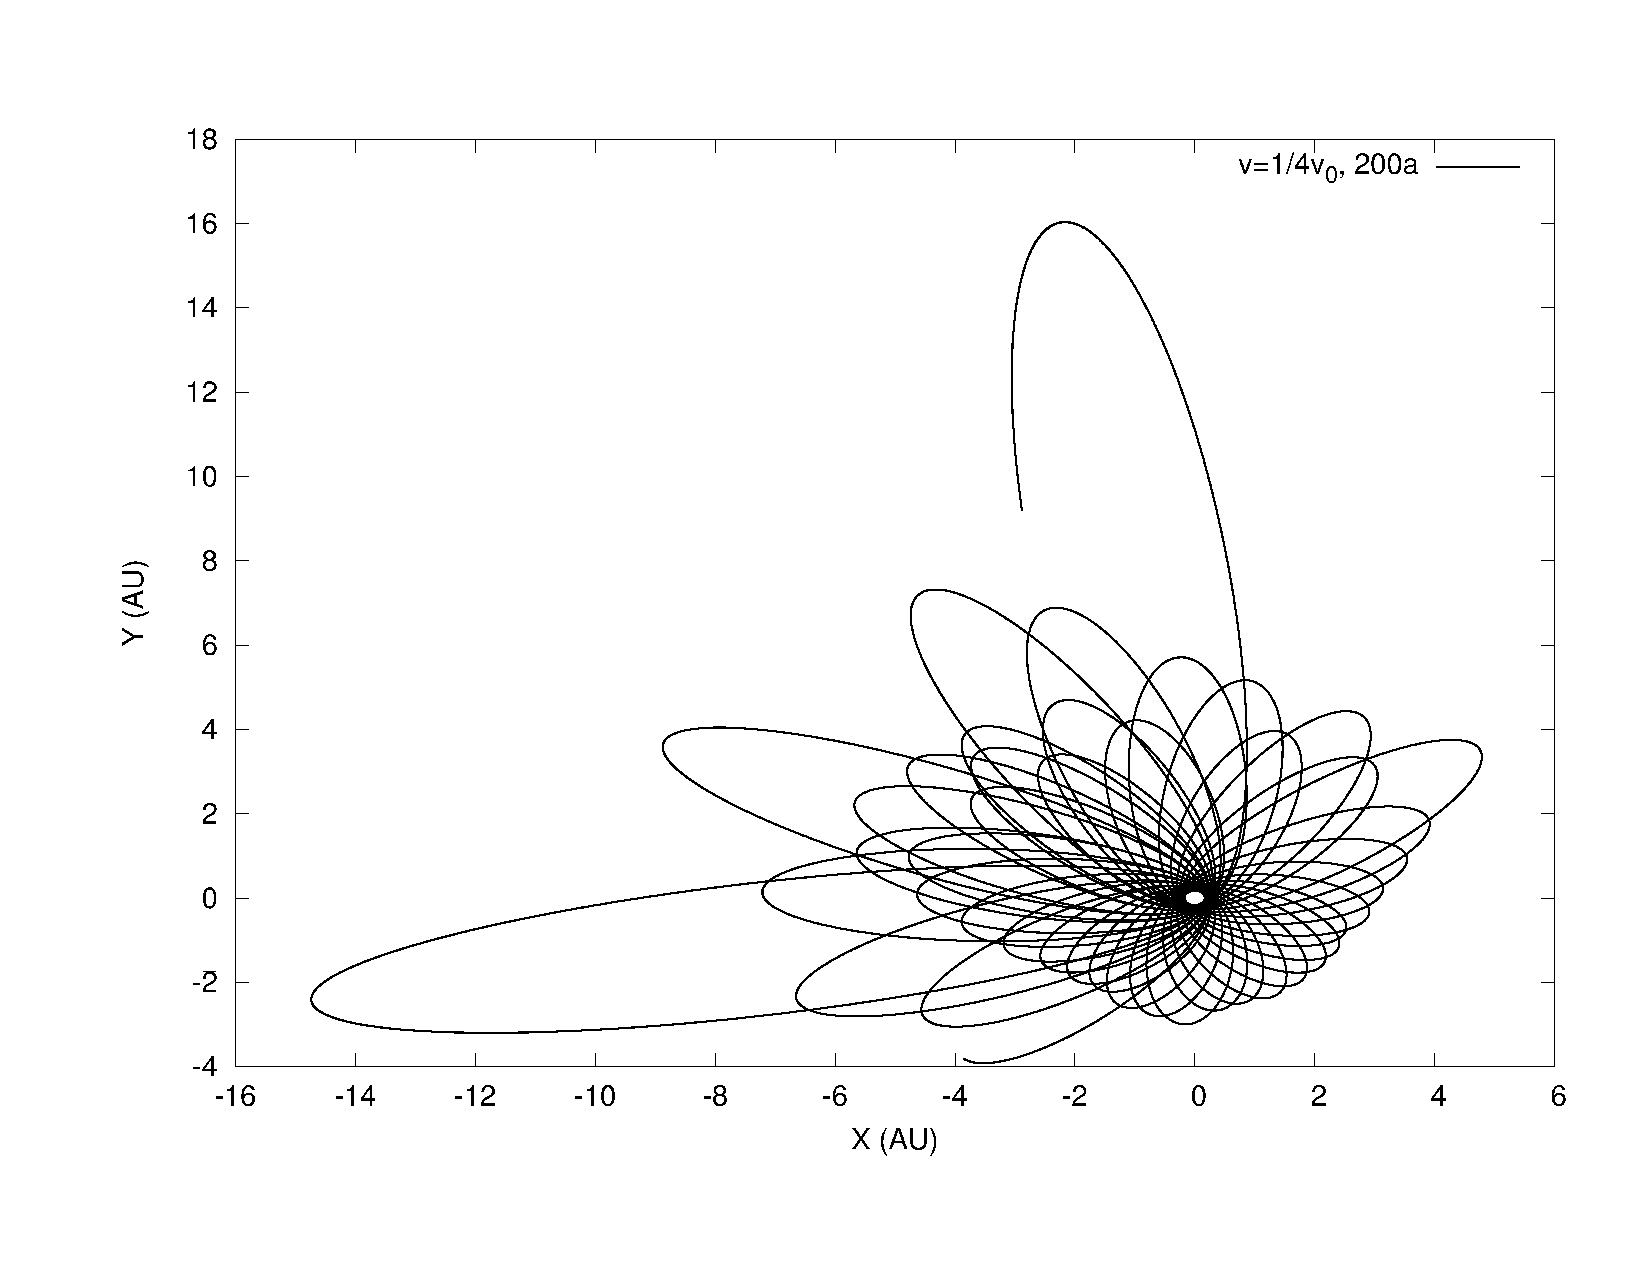
\includegraphics[scale=0.34]{figures/flower}
 \caption{The revolution of Jupiter around the Sun with one fourth starting velocity.}
 \label{fig:jupiter}
\end{center}
\end{figure}

\begin{dialogue}
\speak{Discussion of a plot similar to figure \ref{fig:jupiter}}
\small
\speak{Me} Do one fourth, like you did. [referring to Chris' earlier attempt at one fourth starting velocity]
\speak{John} Nooooo, ok. Aiaiai!
\speak{Me} What happens here? 
\speak{John} Nah, it's hard to say. It gets sucked -- it starts there anyhow -- then it gets sucked in, and then it gets more and more energy?
\speak{Chris} Hmm? It can't get more and more energy?
\speak{John} But it bounces out to here!
\speak{Chris} Yeah, but at that point it's probably got zero velocity. 
\speak{John} Ah, right, I thought about it completely wrong. I'm tired today.
\speak{Chris} 'Cause it aaaalmost hits the Sun. Sweeps past the Sun. Or does it go through? No, it can't do that.
\speak{John} The program would have stopped.
\speak{Chris} Weeeell, would it?
\\ \dots
\speak{John} No, I'm out of ideas. 
\speak{Chris} No, but what happens, there aren't really any errors happening here, is it? It's just that it's being sent abruptly out again after sweeping past the Sun? The Sun bends its path tremendously.
\end{dialogue}

This discussion is somewhat similar to the girls discussion of figure \ref{fig:discrete_acceleration}. Spontaneous concepts from everyday points of view mixed with scientific concepts are uttered in attempts to create meaning behind the plot. The problem, however, is that there's nothing in the model to suggest a change for the orbit over time -- it should stay an ellipse with fixed focal points. Anyhow, as long as the Sun is able to bend Jupiter's path when it sweeps past at a close range, the plot makes sense for the boys. The real problem in this case is the value of the step length being too large. This causes a substantial numerical error to arise when the curve bends abruptly.


\subsection{Meaning making -- dialogue, polyphony and the interplay of concepts}

The positive effects of a good interplay of concepts is already illustrated in section \ref{sec:modes} ``\textit{The math mode}'' section. In that specific case, the boys are recalling scientific concepts in numerical mathematics and, when mediating the concepts on a social plane, they help each other to recall other concepts and to establish these concepts in a physics context for the task at hand. This is typical for the boys' work with the exercises and acts productive in their meaning making process: one mentions an abstract scientific concept and the other connects it to something specific and concrete.

The good effects of dialogic dialogues are quite difficult to exemplify briefly. However, its complete opposite -- the negative effects of an authoritative behavior -- might be just as illustrative. An example can be found in section \ref{sec:modes} ``\textit{The programming mode}'' with the discussion ``\textit{A starting acceleration of 5,5 m/s$^2$ or ...}''. The full discussion is quite long, and starts out with myself asking the question ``who has the right answer?'', to which they answer:

\begin{dialogue}
\small
\speak{Linda} I think you have the right answer.
\speak{Mary} I think I have the right answer as well because it's closer to the original acceleration. 'Cause, an acceleration of 11 is completely insane, isn't it?
\end{dialogue}

\noindent From the beginning, Mary disregards Linda's answer as being ``totally insane''. A bit later in this discussion, in the part recited in section \ref{sec:modes}, Mary still has a clear authoritative point of view, as she doesn't take Linda's uttering of the graph ``falling so fast'' into account. This whole problem gets solved once I intervene and challenge Mary with a falling object-experiment. The comparison of the gravitational acceleration with their thoughts of what a sprinter could achieve, gives Linda the sufficient backing to oppose Mary and get them to actually calculate analytically the acceleration at $t=0$, not just comparing codes and talking about what's most ``natural''. As it turns out, Linda has the right answer.

This last part functions as an example of the importance of polyphony and guidance as well. My voice, in this case in the role of a more capable peer, intervenes and socially mediates a meaningful reference which helps the discussion reach a conclusion. The same is the case with the discussion, also in section \ref{sec:modes} ``\textit{The programming mode}'', on ``\textit{The need of an array?}'' Here, my critically charged questions are enough to get Mary to realize her mistake and come up with the correct answer; a more capable peer's indirect critique of one hypothesis is sufficient to make a new, correct one, emerge.


\section{Implications}
\label{sec:implications}
\subsection{The fragmentation of knowledge: On working in modes and being bound to context}

One of the main challenges for the students seems to be making use of, jumping between and combining different types of skills and knowledge for solving the different problems at hand. The different tasks in the assignments opt for different sets of skills which have been learnt in different contexts: ``comment on the results'', which involves ``talking physics'', might be strongly bound to high school physics (as the only school setting where this has been done until now), while knowledge in programming and discrete mathematics -- which are necessary for discussing the model and modeling in detail -- might be strongly bound to the first semester courses at the University. The new scientific concepts from numerical mathematics and programming are also still under development and might therefore, to some degree, appear fragmented and be in need of more and better connections to relevant spontaneous concepts, e.g. concrete examples of use in physics. One might say that the concepts do not yet ``feel like home'' in the students' physics context.


\subsection{The lack of awareness: Modeling with brand new sets of tools}

When the students are trying to comment on results but fail to reach the correct conclusions, they seem to lack \textit{awareness} on how the new topics in numerical mathematics and programming makes an impact in their work with the assignments. They try to explain odd behavior either with spontaneous concepts or by applying theory from high school physics in a faulty manner. When writing program codes, the easiest way of dealing with problems seems to be by changing code fragments through trial and error. Here, the syntax often gets the blame and the students waste valuable time looking for typographical errors rather than analyzing the mathematical model or the numerical method.

Summarized, the students need to obtain awareness on when and how to use different sets of knowledge and skills and be made aware of the differences between the model and reality. This includes the limitations to the mathematical model and the relevant computer-based limitations. To discuss the model on an adequate level, knowledge in numerical mathematics and programming is essential. These tool sets needs to be actualized in the students' physics context.

\subsection{Developing computational modeling skills}

Good computational modeling skills involve being able to make a plan for working out a model for and simulating some kind of physical system on the computer. This requires sufficient ``algorithmic thinking'', good ``computational scientific thinking'', making use of (sub)goals and several representations and being aware of the different tasks' requirements to different sets of knowledge and skills. Simply doing exercises that includes computational modeling tasks should certainly help the development of these skills. It should also help develop the newly attained scientific concepts from numerical mathematics and informatics in a physics context. 

From a sociocultural point of view, however, this will not occur in an isolated setting but requires collaboration and guidance (by a more capable peer). Left to their own, the students in this study seem to trial and error during programming, focus on calculations when asked to calculate and talk about everyday-physics when asked to comment on results. Instead of using trial and error-methods, they should know more precisely what to do. Instead of using spontaneous everyday concepts when discussing results, they should use scientific concepts and include \textit{the model} with regards to its mathematical form and \textit{computational modeling limitations} in the discussions. These are skills the students need to be made aware are essential for doing computational modeling. Even if the students remember everything they were taught in their first semester, they still need help structuring and applying it correctly in a physics context. One should not expect good modeling skills to emerge on its own having only given the bits and pieces required to do so.


\subsection{The exercise text as the ``skilled modeler'' and narrator of the scientific story}

In line with Vygotsky, the students are in need of someone from whom they may imitate good modeling skills. Ideally, they should be able to imitate the (hypothetical) ``skilled modeler'' (someone with good modeling skills). The students also need help building up ``the scientific story'' of the computational modeling and the physics theory at hand. The narrator of this story should be telling it through an open dialogue with room for alternative hypotheses and multiple points of view (polyphony). Fragmented scientific concepts need to be elaborated and connected to each other and to different specific contexts in their development. Spontaneous concepts need to be decontextualized and applied to more abstract settings.

I propose that, in general, the exercise text has much unused potential of being both the grounds for imitation of good modeling skills and work as a narrator of the scientific story. It demands, however, a certain amount of awareness from the author to write such an exercise text. To allow for imitation, the text should be instructing; it should be written with (sub)goals which ``force'' the students to plan their modeling. To be a good narrator of the scientific story, it should be elaborating and make use of examples to provide meaning behind its theory, instructions and questions. The text should try to help the students grasp the scientific story rather than test if they are able to grasp it on their own, given possibly only a small amount of story fragments.


\begin{acknowledgments}
Big thanks go to Carl Angell and Morten Hjorth-Jensen for their guidance and aid during both the carrying out of the study and the writing of this paper. I would also like to thank Anders Malthe-S\o rensen for letting me lay my critical eyes on his students' work with his carefully designed assignments.
\end{acknowledgments}


\begin{thebibliography}{99}

\bibitem{CMACSE}University of Oslo, The {C}omputers in {S}cience {E}ducation project, <http://www.cma.uio.no/projects/collaborative/\\cse.html>.

\bibitem{Wertsch:1985}James V. Wertsch, \textsl{Vygotsky and the Social Formation of Mind} (Harvard University Press, Cambridge, MA and London, 1985).

\bibitem{Vygotsky:1978}Lev S. Vygotsky, \textsl{Mind in Society} (Harvard University Press, Cambridge, MA, 1978).

\bibitem{Vygotsky:1986}Lev S. Vygotsky, \textsl{Thought and Language} (The MIT Press, Cambridge, MA, 1986).

\bibitem{Wertsch:1991}James V. Wertsch, \textsl{Voices of the Mind} (Harvard University Press, Cambridge, MA, 1991).

\bibitem{Kubli:2005}Fritz Kubli, ``Science Teaching as a Dialogue -- {B}akhtin, {V}ygotsky and some Applications in the Classroom'', Science \& Education {\bf 14} (6), 501--534 (2005).

\bibitem{Mortimer:2003}Eduardo F. Mortimer and Philip H. Scott, \textsl{Meaning Making in Secondary Science Classrooms} (Open University Press, Maidenhead and Philadelphia, 2003).

\bibitem{Ogborn:1996}J. Ogborn, G. Kress, I. Martins and K. McGillicuddy, \textsl{Explaining Science in the Classroom} (Open University Press, Buckingham, 1996).

\bibitem{Hestenes:1992}David Hestenes, Malcolm Wells and Gregg Swackhamer, ``Force Concept Inventory'', The Physics Teacher {\bf 30} (3), 141-158 (1992).

\bibitem{Hestenes:1985}Ibrahim Abou Halloun and David Hestenes, ``Common sense concepts about motion'', Am. J. Phys. {\bf 53} (11), 1056-1065 (1985).

\bibitem{Gautreau:1997}Ronald Gautreau and Lisa Novemsky, ``Concepts first -- A small group approach to physics learning'', Am. J. Phys. {\bf 65}, 418-428 (1997).

\bibitem{Henriksen:2010}Ellen K. Henriksen and Carl Angell, ``The role of `talking physics' in an undergraduate physics class using an electronic audience response system'', Physics Education {\bf 45} (3), 278-284 (2010).

\bibitem{Angell:2004}Carl Angell, ``Exploring students' intuitive ideas based on physics items in {TIMSS} -- 1995,'' Proceedings of the IEA International Research Conference IRC-2004, Cyprus, (2004).

\bibitem{diSessa:1993}Andrea diSessa, ``Towards an Epistemology of Physics'', Cognition and Instruction {\bf 10} (2 and 3), 105-225 (1993).

\bibitem{Mazur:1997}Eric Mazur, \textsl{Peer Instruction} (Prentice Hall, Upper Saddle River, NJ, 1997).

\bibitem{Angell:2008}Carl Angell, Per Morten Kind, Ellen K. Henriksen and {\O}ystein Guttersrud, ``An empirical-mathematical modelling approach to upper secondary physics'', Physics Education {\bf 43} (3), 256-264 (2008).

\bibitem{Futschek:2006}Gerald Futschek, ``Algorithmic Thinking: The Key for Understanding Computer Science'', Lecture Notes in Computer Science {\bf 4226}, 159-168 (2006).

\bibitem{Landau:2006}Rubin Landau, ``Computational Physics -- A Better Model for Physics Education?'', Computing in Science \& Engineering {\bf 8} (5), 22-30 (2006).

\bibitem{Sins:2005}Patrick H. M. Sins, Elwin R. Savelsbergh and Wouter R. van Joolingen, ``The Difficult Process of Scientific Modelling: An analysis of novices' reasoning during computer-based modelling'', International Journal of Science Education {\bf 27} (14), 1695-1721 (2005).

\end{thebibliography}


\end{document}



